\question 若将n阶上三角矩阵A按照列优先顺序存放在一维数组B{[}0,1,,\{n×(n+1)/2\}-1{]}中,第一个非零元素a(1,1)存于B{[}0{]}中,则存放到B{[}k{]}中的非零元素a(i,j)(1≤i≤n,1≤j≤n)的下标i、j与k的对应关系是(
)
\par\twoch{k=i×(i+1)/2+j}{k=i×(i-1)/2+j-1}{k=j×(j+1)/2+i}{\textcolor{red}{k=j×(j-1)/2+i-1}}
\begin{solution}对于元素a(i,j)而言,前面有j-1列,第1列到第j-1列的元素个数分别为1~j-1个,由等差数列求和公式可算得一共有j×(j-1)/2个元素,故k=j×(j-1)/2+i-1(注意B数组是从0开始存元素,因此要减去1)
\end{solution}
\question 设有一个二维数组A{[}m{]}{[}
n{]}在存储中按行优先存放(数组的每一个元素占一个空间),假设A{[}0{]}{[}0{]}存放位置在780(10),A{[}4{]}{[}6{]}存放位置在1146(10),则A{[}6{]}{[}20{]}在(
)位置(其中(10)表明用十进制数表示)
\par\twoch{1342(10)}{1336(10)}{1338(10)}{\textcolor{red}{1340(10)}}
\begin{solution}由Loc(4, 6)=Loc(0,
0)+(4n+6)1=780+(4n+6)=1146,n=(1146-780-6)/4=90,则可计算Loc(6,
20)=Loc(0, 0)+(690+20)1=780+560=1340。
\end{solution}
\question (北京航空航天大学,2004年)若对n阶对称矩阵A以行序为主序方式将其下三角形的元素(包括主对角线上所有元素)依次存放与一维数组B{[}1:n(n+1)/2{]}中,则在B中确定aij(i
\par\twoch{\textcolor{red}{i*(i-1)/2+j}}{j*(j-1)/2+i}{i*(i+1)/2+j}{j*(j+1)/2+i}
\begin{solution}在B中确定aij(i
\end{solution}
\question 将一个A{[}1\ldots{}100,1\ldots{}100{]}的三对角矩阵,按行优先存入一个一维数组B{[}1\ldots{}298{]}中,A中元素A{[}66,65{]}在B中的位置k为(
)
\par\twoch{198}{\textcolor{red}{195}}{197}{199}
\begin{solution}一个三对角矩阵是指一个矩阵aij,其中\textbar{}i-j\textbar{}=0或1,如: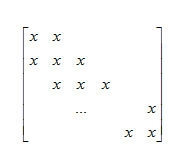
\includegraphics[width=1.93750in,height=1.63542in]{computerassets/2ae8b9b63314226ae69aac4bbb2f4656.png}
所以A中的元素A{[}66,65{]}在B中的位置k为:k=(65-2+1)*3+2+1=195
\end{solution}
